%% For double-blind review submission, w/o CCS and ACM Reference (max submission space)
%\documentclass[sigplan,review,anonymous]{acmart}\settopmatter{printfolios=true,printccs=false,printacmref=false}
%% For double-blind review submission, w/ CCS and ACM Reference
%\documentclass[sigplan,review,anonymous]{acmart}\settopmatter{printfolios=true}
%% For single-blind review submission, w/o CCS and ACM Reference (max submission space)
%\documentclass[sigplan,review]{acmart}\settopmatter{printfolios=true,printccs=false,printacmref=false}
%% For single-blind review submission, w/ CCS and ACM Reference
\documentclass[sigplan,review]{acmart}\settopmatter{printfolios=true}
%% For final camera-ready submission, w/ required CCS and ACM Reference
%\documentclass[sigplan]{acmart}\settopmatter{}


%% Conference information
%% Supplied to authors by publisher for camera-ready submission;
%% use defaults for review submission.
\acmConference[PL'18]{ACM SIGPLAN Conference on Programming Languages}{January 01--03, 2018}{New York, NY, USA}
\acmYear{2018}
\acmISBN{} % \acmISBN{978-x-xxxx-xxxx-x/YY/MM}
\acmDOI{} % \acmDOI{10.1145/nnnnnnn.nnnnnnn}
\startPage{1}

%% Copyright information
%% Supplied to authors (based on authors' rights management selection;
%% see authors.acm.org) by publisher for camera-ready submission;
%% use 'none' for review submission.
\setcopyright{none}
%\setcopyright{acmcopyright}
%\setcopyright{acmlicensed}
%\setcopyright{rightsretained}
%\copyrightyear{2018}           %% If different from \acmYear

%% Bibliography style
\bibliographystyle{ACM-Reference-Format}
%% Citation style
%\citestyle{acmauthoryear}  %% For author/year citations
%\citestyle{acmnumeric}     %% For numeric citations
%\setcitestyle{nosort}      %% With 'acmnumeric', to disable automatic
                            %% sorting of references within a single citation;
                            %% e.g., \cite{Smith99,Carpenter05,Baker12}
                            %% rendered as [14,5,2] rather than [2,5,14].
%\setcitesyle{nocompress}   %% With 'acmnumeric', to disable automatic
                            %% compression of sequential references within a
                            %% single citation;
                            %% e.g., \cite{Baker12,Baker14,Baker16}
                            %% rendered as [2,3,4] rather than [2-4].


%%%%%%%%%%%%%%%%%%%%%%%%%%%%%%%%%%%%%%%%%%%%%%%%%%%%%%%%%%%%%%%%%%%%%%
%% Note: Authors migrating a paper from traditional SIGPLAN
%% proceedings format to PACMPL format must update the
%% '\documentclass' and topmatter commands above; see
%% 'acmart-pacmpl-template.tex'.
%%%%%%%%%%%%%%%%%%%%%%%%%%%%%%%%%%%%%%%%%%%%%%%%%%%%%%%%%%%%%%%%%%%%%%


%% Some recommended packages.
\usepackage{booktabs}   %% For formal tables:
                        %% http://ctan.org/pkg/booktabs
\usepackage{subcaption} %% For complex figures with subfigures/subcaptions
                        %% http://ctan.org/pkg/subcaption
\usepackage{listings}
\usepackage{upquote}

\usepackage{color}
\definecolor{bluekeywords}{rgb}{0.13,0.13,1}
\definecolor{greencomments}{rgb}{0,0.5,0}
\definecolor{redstrings}{rgb}{0.9,0,0}

\lstdefinelanguage{FSharp}%
{morekeywords={let, new, match, with, rec, open, module, namespace, type, of, member, % 
and, for, while, true, false, in, do, begin, end, fun, function, return, yield, try, %
mutable, if, then, else, cloud, async, static, use, abstract, interface, inherit, finally },
  otherkeywords={ let!, return!, do!, yield!, use!, var, from, select, where, order, by },
  keywordstyle=\color{bluekeywords},
  sensitive=true,
  basicstyle=\ttfamily,
  breaklines=true,
  xleftmargin=\parindent,
  aboveskip=\bigskipamount,
  tabsize=4,
  morecomment=[l][\color{greencomments}]{///},
  morecomment=[l][\color{greencomments}]{//},
  morecomment=[s][\color{greencomments}]{{(*}{*)}},
  morestring=[b]",
  showstringspaces=false,
  literate={`}{\`}1,
  stringstyle=\color{redstrings},
}

\begin{document}

%% Title information
\title[]{Extended Abstract: F\# OpenCL Type Provider}         %% [Short Title] is optional;
                                        %% when present, will be used in
                                        %% header instead of Full Title.
% \titlenote{with title note}             %% \titlenote is optional;
                                        %% can be repeated if necessary;
                                        %% contents suppressed with 'anonymous'
% \subtitle{Subtitle}                     %% \subtitle is optional
% \subtitlenote{with subtitle note}       %% \subtitlenote is optional;
                                        %% can be repeated if necessary;
                                        %% contents suppressed with 'anonymous'


%% Author information
%% Contents and number of authors suppressed with 'anonymous'.
%% Each author should be introduced by \author, followed by
%% \authornote (optional), \orcid (optional), \affiliation, and
%% \email.
%% An author may have multiple affiliations and/or emails; repeat the
%% appropriate command.
%% Many elements are not rendered, but should be provided for metadata
%% extraction tools.

\author{Kirill Smirenko}

\affiliation{
%  \position{Position2a}
%  \department{Department2a}             %% \department is recommended
  \institution{St.Petersburg State University}           %% \institution is required
  \streetaddress{Universitetski pr., 28}
  \city{St.Petersburg}
  \postcode{198504}
  \country{Russia}                   %% \country is recommended
}
\email{k.smirenko@gmail.com}         %% \email is recommended

%% Author with single affiliation.
\author{Semyon Grigorev}
%\authornote{Saint Petersburg State University}          %% \authornote is optional;
                                        %% can be repeated if necessary
\orcid{0000-0002-7966-0698}             %% \orcid is optional
\affiliation{
  \position{Associate Professor}
  \institution{St.Petersburg State University}           %% \institution is required
  \streetaddress{Universitetski pr., 28}
  \city{St.Petersburg}
  \postcode{198504}
  \country{Russia}                   %% \country is recommended
}
\email{semen.grigorev@jetbrains.com}          %% \email is recommended


%% Abstract
%% Note: \begin{abstract}...\end{abstract} environment must come
%% before \maketitle command
\begin{abstract}
The popularity of GPGPU usage in applied software is growing but GPGPU utilization in high-level programming languages is still challenged.
We present an F\# type provider: a way to use existing OpenCL C source code in F\# in a strongly typed way. 
\end{abstract}


%% 2012 ACM Computing Classification System (CSS) concepts
%% Generate at 'http://dl.acm.org/ccs/ccs.cfm'.
\begin{CCSXML}
<ccs2012>
<concept>
<concept_id>10011007.10011006.10011008.10011009.10011012</concept_id>
<concept_desc>Software and its engineering~Functional languages</concept_desc>
<concept_significance>500</concept_significance>
</concept>
<concept>
<concept_id>10011007.10011006.10011008.10011009.10010175</concept_id>
<concept_desc>Software and its engineering~Parallel programming languages</concept_desc>
<concept_significance>100</concept_significance>
</concept>
</ccs2012>
\end{CCSXML}
\ccsdesc[500]{Software and its engineering~Functional languages}
\ccsdesc[100]{Software and its engineering~Parallel programming languages}%% End of generated code


%% Keywords
%% comma separated list
\keywords{Type Providers, Metaprogramming, Generic Programming, GPGPU, OpenCL}  %% \keywords are mandatory in final camera-ready submission


%% \maketitle
%% Note: \maketitle command must come after title commands, author
%% commands, abstract environment, Computing Classification System
%% environment and commands, and keywords command.
\maketitle


\section{Introduction} % in progress

General Purpose Graphical Processor Units, or GPGPUs, are commonly used for fast computations. Their multi-core architecture benefits high-load computations in applied science, computer vision, bioinformatics and other areas~\cite{CUDA_to_OpenCL, GPGPU_1}.

Several frameworks for GPGPU programming are known. The most popular one is CUDA, a platform for parallel GPGPU computations developed by Nvidia in 2007~\cite{CUDA}. Another important project is Open Computing Language (OpenCL), an open standard for cross-platform parallel computing on different platforms, including GPGPU~\cite{OpenCL}. CUDA and OpenCL functions executed on a GPGPU device are called \textit{kernels}.

The technologies mentioned provide special programming languages: CUDA C/C++, OpenCL C/C++. However using higher-level languages, such as C\# or F\#, can be more convenient for GPGPU development for the following reasons: they are used more often for general software development, and they are strongly and statically typed, which, with the help of integrated development environments (IDEs), facilitates development and improves the reliability of software. In this article, in context of GPGPU development, we are going to call programming in special CUDA/OpenCL languages \textit{lower-level development}, and coding in C\#/F\# \textit{higher-level development}.

There are several instruments for higher-level GPGPU development. AleaGPU~\cite{AleaGPU} is a commercial product that allows using C\# and F\# for CUDA programming, and calling a limited number of included lower-level CUDA libraries. The work~\cite{FSCL} presents FSCL, a limited subset of F\# to OpenCL compiler, which allows developing OpenCL kernels within the .NET environment.
Brahma.FSharp~\cite{Brahma_FSharp} is another F\# to OpenCL compiler, but it differs from FSCL in that it focuses on translating F\# \textit{quotations}, not regular code.
F\# quotations are specific expressions that are not compiled as part of a program, but instead are compiled into objects that represent F\# expressions, and can be evaluated later with F\# language tools.
Moreover, Brahma.FSharp is under active development, while FSCL has not been updated since January 2016.

There are also tools for managing GPGPU code launches from .NET. As mentioned earlier, Alea GPU allows reusing some CUDA libraries. CUSP~\cite{CUSP} is a C++ library that enhances CUDA development with sparse linear algebra and graph computations. ManagedCUDA~\cite{ManagedCUDA} library allows to run arbitrary pre-compiled CUDA kernels from C\#, however the calls are untyped, which doesn't satisfy the need for a completely type-safe environment.

To our knowledge, neither of the existing solutions allows both programming for GPGPU in higher-level programming languages and calling arbitrary OpenCL C code in a strongly typed way. In our work we are trying to solve this problem by augmenting Brahma.FSharp project with a new component that loads OpenCL C source files with a mechanism called type provider.

\section{F\# type providers}

A type provider~\cite{syme2012strongly} (TP) is a component of F\# programming language that provides types, properties, and methods during runtime~\cite{TypeProviders}. One major application of F\# type providers is integration with dynamic data sources, such as SQL, CSV, JSON, in a strongly typed way~\cite{FSharpData}. Type providers can have static parameters and thus receive configuration, data source etc. as arguments. Therefore, type providers allow the user to interact with data from dynamic sources (such as a file) in a statically typed way.

One relevant example is R~Type Provider~\cite{R_TP}. It enables interoperability between F\# and R by discovering installed R packages and making them available as .NET namespaces underneath the parent namespace RProvider. Another example is SQL Type Provider~\cite{SQL_TP} that connects the F\# environment in IDE to database sources and allows to explore them in a type-safe manner.

A common alternative to type providers is code generation. However, type providers ensure better integration with user context because they work at runtime, while the generated code must be replaced each time the data source is modified. Thus the threat of dissynchronization with the data source is eliminated.

Type providers also have disadvantages. First of all, testing type providers is very challenging because an IDE instance with any code that uses a TP, including unit tests, locks the DLL that contains the type providers and thus prevents rebuilding it. Also, debugging a type provider is a challenging process that requires two IDE instances and unusual setup, and editing TP is still impossible until the other IDE instance is closed.

\section{OpenCL type provider}

In order to simplify usage of existing OpenCL C kernels in applied software, we propose the OpenCL type provider which is implemented as a part of Brahma.FSharp and works as follows. 
The type provider loads the specified OpenCL C file, performs lexing and parsing of the loaded file, and generates an F\# type with static functions that have the same signatures as the original OpenCL functions.
After that one can use provided functions in code quotations to be compiled by Brahma.FSharp to OpenCL C.

To use OpenCL type provider in a project, the user has to include the DLL containing the TP.
Then, the KernelProvider type should be initialized with the proper static parameters, which there are two: \textit{PathToFile} specifies the path to the OpenCL C source file being included;
\textit{TreatPointersAsArrays} defines whether the function parameters in OpenCL source code that are pointers are represented in F\# environment with the corresponding array type or reference type (ByRef in F\#).


The generated type provides all functions from the OpenCL C file as static F\# functions.
Listing~\ref{lst:usage} shows an example of TP usage: the file \textit{mygemm.cl} is included, and the function \lstinline{myGEMM1} from that file is generated within the provided type in F\#.

%\begin{figure}[h]
%\centering
%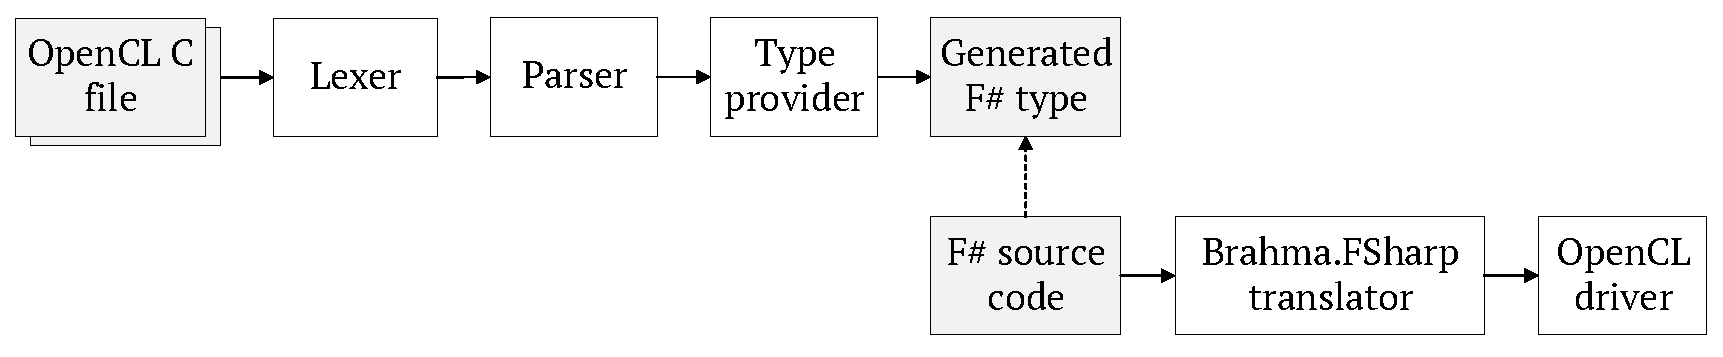
\includegraphics[width=8.5cm]{graphics/architecture.pdf}
%\caption{Overview of the solution}
%\label{architecture}
%\end{figure}

% \begin{figure}[h]
% \centering
% 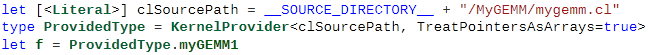
\includegraphics[width=8.5cm]{graphics/example-usage.png}
% \caption{Example: TP usage}
% \label{pic:usage}
% \end{figure}

\lstset{language=FSharp}
\begin{lstlisting}[
  caption={Example of TP usage},
  label=lst:usage,
  basicstyle=\footnotesize,%\tiny, %or \small or \footnotesize etc.
  captionpos=b
]
let [<Literal>] clSourcePath = __SOURCE_DIRECTORY__ + "/MyGEMM/mygemm.cl"
type Provided = KernelProvider<clSourcePath, TreatPointersAsArrays=true>
let cmd = <@ fun ... -> Provided.myGEMM1 ... @>
\end{lstlisting}

The screenshots below show examples of how the proposed type provider enhances the development process. Type information of the reused code becomes available (figure~\ref{pic:intellisense}), as well as code suggestions (figure~\ref{pic:suggestions}). Compile-time type check of interactions with the reused code is performed (figure~\ref{pic:error}).

\begin{figure}[h]
\centering
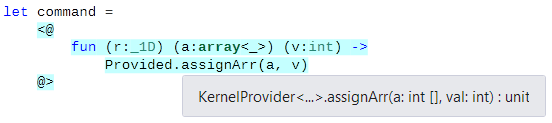
\includegraphics[width=8.5cm]{graphics/example-suggestion.png}
\caption{Type information in IDE}
\label{pic:intellisense}
\end{figure}

\begin{figure}[h]
\centering
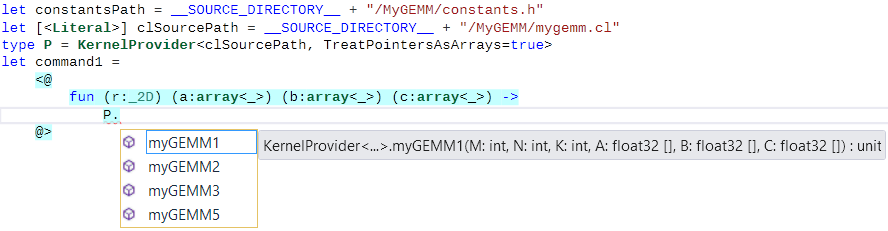
\includegraphics[width=8.5cm]{graphics/example-multiple-suggestions.png}
\caption{Code suggestions in IDE}
\label{pic:suggestions}
\end{figure}

\begin{figure}[h]
\centering
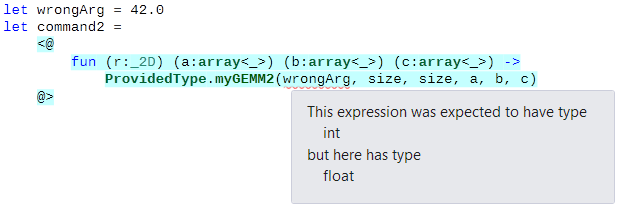
\includegraphics[width=8.5cm]{graphics/example-compile-error.png}
\caption{Compile-time type check with TP}
\label{pic:error}
\end{figure}

\section{Discussion}
                                                                                                                                                                                
Our solution works on .NET and Mono (for Mac and Linux) and published as part of NuGet pachage~\cite{Brahma.FSahrp.NuGet}.

We can propose some possible directions for the future work. First of all, it is necessary to improve OpenCL C parser and translator which are used in type provider.
It is required for complex kernels handling and also for more deep and transperent integration of OpenCL C and F\# type systems.
For example, running OpenCL code on different devices requires proper configuration of parameters such as grid size and tile size. 
Brahma.FSharp allows to set grid parameters but does not allow to pass arbitrary constants. 
Therefore, header files (.h) containing \lstinline{#define} preprocessor macros may be required along with the reused OpenCL C code. 
We hope to find a way to mitigate this restriction in the future.

Another direction is a unification of kernel primitive provided by Brahma.Fsharp and kernels loaded by TP.
It looks natural for an end user to think that kernel primitive from Brahma.FSahrp and OpenCL C kernel can be used in the same manner, but currently, we have two different representations for them.

%% Acknowledgments
\begin{acks}
The research was supported by a grant from \grantsponsor{}{JetBrains Research}{https://research.jetbrains.org/}.
\end{acks}
%                            %% acks environment is optional
%                                         %% contents suppressed with 'anonymous'
%   %% Commands \grantsponsor{<sponsorID>}{<name>}{<url>} and
%   %% \grantnum[<url>]{<sponsorID>}{<number>} should be used to
%   %% acknowledge financial support and will be used by metadata
%   %% extraction tools.
%   This material is based upon work supported by the
%   \grantsponsor{GS100000001}{National Science
%     Foundation}{http://dx.doi.org/10.13039/100000001} under Grant
%   No.~\grantnum{GS100000001}{nnnnnnn} and Grant
%   No.~\grantnum{GS100000001}{mmmmmmm}.  Any opinions, findings, and
%   conclusions or recommendations expressed in this material are those
%   of the author and do not necessarily reflect the views of the
%   National Science Foundation.

%% Bibliography
\bibliography{ext-abstract}

%% Appendix
% \appendix
% \section{Appendix}

% Text of appendix \ldots

\end{document}
